\documentclass[a4paper]{article}

%% Language and font encodings
\usepackage[english]{babel}
\usepackage[utf8x]{inputenc}
\usepackage[T1]{fontenc}

%% Sets page size and margins
\usepackage[a4paper,top=3cm,bottom=2cm,left=3cm,right=3cm,marginparwidth=1.75cm]{geometry}

%% Useful packages
\usepackage{amsmath}
\usepackage{graphicx}
\usepackage[colorinlistoftodos]{todonotes}
\usepackage[colorlinks=true, allcolors=blue]{hyperref}
\usepackage{listings}
\usepackage{xcolor}
\usepackage{fancyvrb, newverbs, color}

\lstset { %
    language=C++,
    basicstyle=\footnotesize,% basic font setting
    keywordstyle=\color{blue}\ttfamily,
    stringstyle=\color{red}\ttfamily,
    commentstyle=\color{green}\ttfamily,
    morecomment=[l][\color{magenta}]{\#}
}

\title{Udacity Flying Car Nanodegree 3rd Project\\ 
       Implement Controllers in C++}
\author{Xinjie Qiu \\
		qiuxinjie@gmail.com}
\date{\today}

\begin{document}
\maketitle

\section{Introduction}

The purpose of this project is to write low level controllers for the flight vehicle in C++. This includes implementing controller and tuning control gains. 

\section{Drone Controllers}

To control the drone in three dimension, the following controller architecture is adopted, which consists of \textbf{att}itude controller, \textbf{alt}itude controller, lateral controller. The attitude controller breaks down into smaller controllers responsible for body rate, roll-pitch, and yaw. There are total of 5 controllers to implement in this project. 

\begin{figure}[ht]
\centering
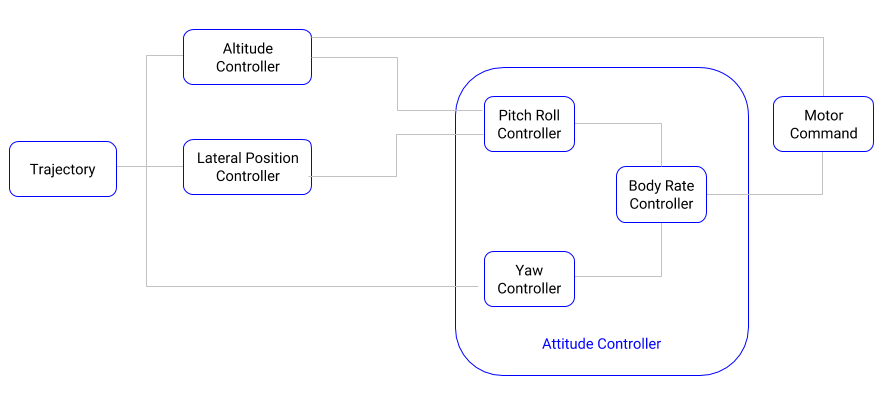
\includegraphics[width=0.9\textwidth]{./fig/ControlArchitecture.png}
\caption{\label{fig:controller} overall control architecture.}
\end{figure}

In the following subsections, each controller will be implemented in C++.

\subsection{body rate control} \label{control:bodyrate}

Body rate controller is implemented as a P (proportional) controller. It collects commanded roll, pitch, and yaw rates ($p, q, r$), then translates into the desired commanded moments along the axis. 

The control equations have the following form:
$$ \dot{\omega}_{p} = k_{p}^{P} (p_c - p) $$
$$ \dot{\omega}_{q} = k_{p}^{Q} (q_c - q) $$
$$ \dot{\omega}_{r} = k_{p}^{R} (r_c - r) $$
Note, throughout this document, quantity with subscript c means a "commanded" (or "desired") one, without subscript means an "actual" (or more precisely speaking, "estimated") one.

The commanded moments (M, or torque $\tau$ in physics, in unit [$N \cdot m$]) is the product of moment of inertia ($I$, [$kg \cdot m^2$]) and angular acceleration ($\dot{\omega}$, [$radians/s^2$]).
$$ M = I \dot{\omega} $$
The implemented body rate controller is:

\begin{lstlisting}[frame=single]
	V3F momentCmd;
	V3F rate_error = pqrCmd - pqr;
	V3F omega_dot_des = rate_error * kpPQR;
	momentCmd = omega_dot_des * V3F(Ixx, Iyy, Izz);
\end{lstlisting}

\subsection{roll pitch control} \label{control:rollpitch}
The roll-pitch controller is the trickiest controller to implement due to that it involves rotation matrix from inertial frame to body frame. It is a P controller responsible for commanding the roll and pitch rates in the body frame. It uses the lateral acceleration and thrust commands, in addition to the vehicle attitude to output a body rate command. 

The controller first calculates the acceleration in the thrust direction in the body frame $c_d$ from dividing the collective thrust by drone's mass. Then the target angles are calculated from local accelerations. Note both target angles need to be constraint within maximum title angle.
\begin{gather*}
R_{13c} = b^x_c = - \ddot{x} / c_d \\
R_{23c} = b^y_c = - \ddot{y} / c_d
\end{gather*}
The reason there is a minus sign is due to that the vertical component of thrust is negative in the NED coordinate system.

The desired body rates are then set the rate of change of the given matrix elements using a P controller,
$$\dot{b}^x_c  = k_p^{bank}(b^x_c - b^x)$$
$$\dot{b}^y_c  = k_p^{bank}(b^y_c - b^y)$$
where $b^x = R_{13}$ and $b^y = R_{23}$. The given values can be converted into the angular velocities in the body frame by the matrix multiplication. 

$$
\begin{pmatrix} p_c \\ q_c \\ \end{pmatrix}  = \frac{1}{R_{33}}\begin{pmatrix} R_{21} & -R_{11} \\ R_{22} & -R_{12} \end{pmatrix} \begin{pmatrix} \dot{b}^x_c \\ \dot{b}^y_c  \end{pmatrix} 
$$

\begin{lstlisting}[frame=single]
    V3F pqrCmd;
    Mat3x3F R = attitude.RotationMatrix_IwrtB();
    
    float c_d = collThrustCmd/mass;
    float R13_c = CONSTRAIN(-accelCmd.x/c_d, -maxTiltAngle, maxTiltAngle);
    float R23_c = CONSTRAIN(-accelCmd.y/c_d, -maxTiltAngle, maxTiltAngle);
    float bx_dot_cmd = kpBank*(R13_c - R(0,2));
    float by_dot_cmd = kpBank*(R23_c - R(1,2));
    pqrCmd.x = (R(1,0)*bx_dot_cmd - R(0,0)*by_dot_cmd)/R(2,2);
    pqrCmd.y = (R(1,1)*bx_dot_cmd - R(0,1)*by_dot_cmd)/R(2,2);
    pqrCmd.z = 0.0;
\end{lstlisting}

\subsection{altitude controller} \label{control:altitude}

In this altitude controller implementation, velocity uses a feed forward P controller,
$$\dot{z} = \dot{z}_c  + k_{p}^{posZ}(z_{c} - z) $$
This vertical component of velocity is constraint between maximum ascent rate and maximum descent rate.

Acceleration uses a feed forward PI controller, which also contains an integrator part to handle the non-ideal center of gravity presented in scenario 4,
$$\ddot{z} = \ddot{z}_c + k_{p}^{velZ}(\dot{z}_{c} - \dot{z}) + k_i^{posZ}\int_0^t(z_{c} - z)dt'$$ 

In the altitude controller, the thrust is controlled through the vertical acceleration. From Newton's second law of motion, the acceleration in z direction is,
$$ m \ddot{z} = - F_{thrust} b^z + m g$$
$g$ is in positive direction, thrust is in negative direction in the NED system. $b^z = R_{33}$ are the the last row last column element in the rotation matrix to translate back from inertial frame to body frame in the case of non-zero roll/pitch angles.
$$ F_{thrust} = m (g - \ddot{z})/b^z$$ 

The C++ implementation code:
\begin{lstlisting}[frame=single]
    float velocityZ = kpPosZ * (posZCmd - posZ) + velZCmd;
    // Limit the ascent/descent rate
    velocityZ = CONSTRAIN(velocityZ, - maxAscentRate, maxDescentRate);
    
    integratedAltitudeError += (posZCmd - posZ) * dt;
    
    float accelerationZ =  accelZCmd
                    + kpVelZ * (velocityZ - velZ)
                    + KiPosZ * integratedAltitudeError;
    
    thrust = mass * (CONST_GRAVITY - accelerationZ) / R(2,2);

\end{lstlisting}

\subsection{lateral position control} \label{control:lateral}
The lateral position control uses two cascaded feedforward linear P controller to generate a commanded local acceleration from the local north/east position, velocity and acceleration.

$$\dot{x} = \dot{x}_c  + k_{p}^{PosXY}(x_{c} - x), \:
  \dot{y} = \dot{y}_c  + k_{p}^{PosXY}(y_{c} - y)$$
$$\ddot{x} = \ddot{x}_c  + k_{p}^{VelXY}(\dot{x_{c}} - \dot{x}), \:
  \ddot{y} = \ddot{y}_c  + k_{p}^{VelXY}(\dot{x_{c}} - \dot{y})$$

\textit{I tried to constraint maximum XY velocity and maximum XY acceleration. But in the later gain tuning part, these constraints prevent the green drone in the $4^{th}$ scenario to reach its target location. For now, I just lift these constraints.}

\begin{lstlisting}[frame=single]
    V3F velocity_xy = velCmd + kpPosXY*(posCmd-pos);
    // Limit speed
    // if (velocity_xy.mag() > maxSpeedXY)
    //        velocity_xy = velocity_xy.norm() * maxSpeedXY;
    
    accelCmd = accelCmd + kpVelXY*(velocity_xy - vel);
    // limit accelaration
    // if (accelCmd.mag() > maxAccelXY)
    //     accelCmd = accelCmd.norm() * maxAccelXY;
\end{lstlisting}

\subsection{yaw control} \label{control:yaw}
The yaw controller is a linear proportional heading controller to yaw rate commands.
The control over yaw is decoupled from the all other directions.
$$ r_c = k_p^{yaw} (\psi_c - \psi) $$

\begin{lstlisting}[frame=single]
    yawCmd = fmodf(yawCmd,M_PI*2.0);
    float yaw_error = AngleNormF(yawCmd - yaw);
    yawRateCmd = kpYaw*yaw_error;
\end{lstlisting}

\subsection{calculate the motor commands given commanded thrust and moments} \label{control:motorcommand}

Using the desired or estimated position, velocity, attitude, and body rates information sent from the simulator, commands are passed from the above 5 controllers as three directional body moments and thrust. These desired 3-axis moment and collective thrust command are then converted to individual motor thrust commands.

The numbering order of propellers in the C++ project is displayed in figure~\ref{fig:drone1}. 1 is front left, 2 is front right, 3 is rear left, 4 is rear right. Notice this numbering order is different from the lecture exercise and the Python project. Specifically, 3 and 4 are switched. 

\begin{figure}[ht]
\centering
\includegraphics[width=0.5\textwidth]{./fig/drone1.png}
\caption{\label{fig:drone1} Propeller location.}
\end{figure}

Distance from vehicle origin to motors is $L$, the distance from motor to x or y axis is $ l = L/\sqrt[]{2}$. The thrust from each propeller is labeled as $F_1$, $F_2$, $F_3$, $F_4$, the collective thrust is
$$ F_{total} = F_1 + F_2 + F_3 + F_4 $$
For roll motion, the moments generated by the $1^{st}$ and $3^{rd}$ propellers are counteracted by the moment generated by the $2^{nd}$ and the $4^{th}$ propellers. 
$$ \tau_x = (F_1 - F_2 + F_3 - F_4)l $$
In the same fashion, the pitch is generated by the mismatch of the moments created by $1^{st}$ and $2^{nd}$ propellers and the moment generated by the $3^{rd}$ and $4^{th}$ propellers.
$$ \tau_y = (F_1 + F_2 - F_3 - F_4)l $$
Contrary to the roll and pitch, the yaw motion is executed by the mismatch of the moments generated by the propellers along the z axis by the reactive force. The moment generated by the propeller is directed opposite of its rotation and is proportional to the square of the angular velocities. The propellers 1 and 4 rotate in clockwise thus producing the moment in the counterclockwise direction with negative moments. Propellers 2 and 3 rotate in counterclockwise thus the resulting moments are in opposite and have the positive moments.
\begin{align*}
\tau_z &= k_m (-\omega^2_1 + \omega^2_2 + \omega^2_3 - \omega^2_4) \\
       &= -\frac{k_m}{k_f} (F_1 - F_2 - F_3 + F_4) \\
       &= -k_{appa}  (F_1 - F_2 - F_3 + F_4)
\end{align*}

Rearrange these 4 equations, we have
\begin{align*}
F_1 + F_2 + F_3 + F_4 &= F_{total}  \\
F_1 - F_2 + F_3 - F_4 &= \tau_x / l \\
F_1 + F_2 - F_3 - F_4 &= \tau_y / l \\
F_1 - F_2 - F_3 + F_4 &= -\tau_z / k_{appa}
\end{align*}

Quantities on the left side are unknown, on the right side are konwn. Solve these 4 equations for thrust from each propeller,
\begin{align*}
F_1 = (F_{total} + \tau_x / l + \tau_y / l  -\tau_z / k_{appa})/4  \\
F_2 = (F_{total} - \tau_x / l + \tau_y / l  +\tau_z / k_{appa})/4 \\
F_3 = (F_{total} + \tau_x / l - \tau_y / l  +\tau_z / k_{appa})/4 \\
F_4 = (F_{total} - \tau_x / l - \tau_y / l  -\tau_z / k_{appa})/4
\end{align*}

Motor command implementation in C++:
\begin{lstlisting}[frame=single]
    float lenth = L / sqrtf(2);
    float F_total = collThrustCmd;
    float F_x     = momentCmd.x / lenth;
    float F_y     = momentCmd.y / lenth;
    float F_z     = - momentCmd.z / kappa;
    cmd.desiredThrustsN[0] = (F_total + F_x + F_y + F_z) / 4.f; // front left, [N]
    cmd.desiredThrustsN[1] = (F_total - F_x + F_y - F_z) / 4.f; // front right
    cmd.desiredThrustsN[2] = (F_total + F_x - F_y - F_z) / 4.f; // rear left
    cmd.desiredThrustsN[3] = (F_total - F_x - F_y + F_z) / 4.f; // rear right
\end{lstlisting}

\section{Flight Control Gain Tuning}

Now we have all pieces of code for each controller. Let's fire up the simulator to test them out, and tune these control gain parameters in QuadControlParams.txt.

\subsection{Scenario 1: Intro}

In the first scenario we want to make the vehicle more or less stay in the same spot. Because in the starter code, thrust of each propeller is simply being set to: $QuadControlParams.Mass*9.81/4$.

To make drone not falling to the ground, drone's gravity need to be compensated from propeller's thrust force. All we have to do is to adjust the Mass control parameter in QuadControlParams.txt to match the physical property mass in QuadPhysicalParams.txt. Changing $Mass = 0.5$ is all it takes to stabilize the drone. Scenario 1 picture from simulator is shown in Figure~\ref{fig:scenario1}.

\begin{figure}[ht]
\centering
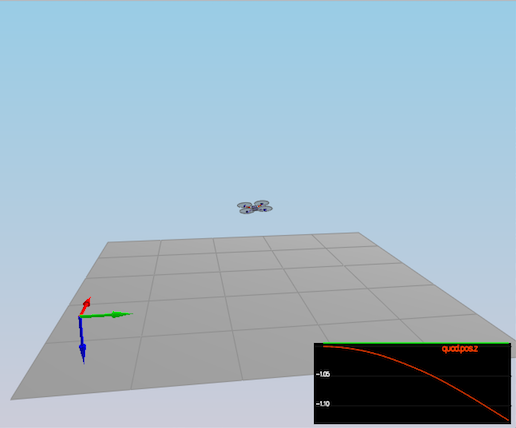
\includegraphics[width=0.5\textwidth]{./fig/scenario1.png}
\caption{\label{fig:scenario1} Scenario 1 Tuning Mass.}
\end{figure}

\subsection{Scenario 2: Body rate and roll/pitch control}

Scenario 2 in the simulator is to help check the correctness of the body rate and roll/pitch controller implementation. It also helps to tune control gain parameters for these controllers.

The following functions need to be implemented, and the gains need to be tuned: 
\begin{description}

\item [GenerateMotorCommands()] The motor command implementation can be found in subsection~\ref{control:motorcommand}. No gain tuning for this function.

\item [BodyRateControl()] The body rate control implementation can be found in subsection~\ref{control:bodyrate}. Tuning kpPQR helps to get the vehicle to stop spinning quickly once the rotation of the vehicle about roll (omega.x) get controlled to zero. The default kpPQR gains work for this scenario, no need to change them.
\begin{Verbatim}[frame=single]
# Angle rate gains
kpPQR = 23, 23, 5
\end{Verbatim} 

\item [RollPitchControl()] The roll pitch control implementation can be found in subsection~\ref{control:rollpitch}. Tune kpBank minimize settling time and avoid too much overshoot. Quad level itself and vehicle angle (Roll) get controlled to zero. Gain kpBank need to tune up from 5 to 8 for this scenarios.
\begin{Verbatim}[frame=single,commandchars=\\\{\}]
# Angle control gains
kpBank = \textcolor{red}{8}
\end{Verbatim} 

\end{description}

After the gain tuning, the simulator output the following test result:
\begin{Verbatim}[frame=lines, label=Simulator Test Result Output, commandchars=\\\{\}]

Simulation #751 (../config/2_AttitudeControl.txt)
\textcolor{green}{PASS}: ABS(Quad.Roll) was less than 0.025000 for at least 0.750000 seconds
\textcolor{green}{PASS}: ABS(Quad.Omega.X) was less than 2.500000 for at least 0.750000 seconds
\end{Verbatim} 

\begin{figure}[ht]
\centering
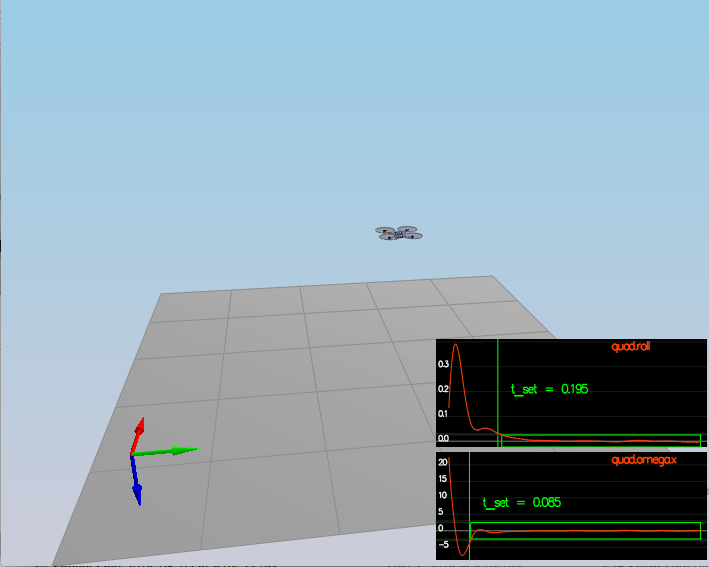
\includegraphics[width=0.5\textwidth]{./fig/scenario2.png}
\caption{\label{fig:scenario2} Scenario 2 Body rate and roll/pitch control.}
\end{figure}

\subsection{Scenario 3: Position/velocity and yaw angle control}

Scenario 3 in the simulation helps to test the implementation of the position, altitude and yaw control for the quad. Two identical quads are created, one offset from its target point with yaw initialized to 0, the second offset from target point with yaw = 45 degrees.

\begin{description}
\item [LateralPositionControl()] The code for lateral position  control is implemented in~\ref{control:altitude}. 

\item [AltitudeControl()] The code for altitude control is implemented in~\ref{control:lateral}. 

Tuning parameters kpPosZ, kpVelZ, kpVelXY and kpVelXY find out only kpPosXY need to be changed from 1 to 2 to make the quads go to their destination points and tracking error go down. 

\begin{Verbatim}[frame=single,commandchars=\\\{\}]
# Position control gains
kpPosZ = 1
kpPosXY = \textcolor{red}{2}
# Velocity control gains
kpVelXY = 4
kpVelZ = 4
\end{Verbatim} 

However, one quad remains rotated in yaw. It requires the yaw control in the next paragraph. 

\item [YawControl()] The code for yaw control is implemented in~\ref{control:yaw}. Tuning parameters kpYaw from 1 to 2 makes the simulation pass the yaw control test.
% and the 3rd (z) component of kpPQR. 
% Tune position control for settling time. 

\begin{Verbatim}[frame=single,commandchars=\\\{\}]
# Angle control gains
kpYaw = \textcolor{red}{2}
\end{Verbatim} 

\end{description}

\begin{Verbatim}[frame=lines, label=Simulator Test Result Output, commandchars=\\\{\}]

Simulation #1128 (../config/3_PositionControl.txt)
\textcolor{green}{PASS}: ABS(Quad1.Pos.X) was less than 0.100000 for at least 1.250000 seconds
\textcolor{green}{PASS}: ABS(Quad2.Pos.X) was less than 0.100000 for at least 1.250000 seconds
\textcolor{green}{PASS}: ABS(Quad2.Yaw) was less than 0.100000 for at least 1.000000 seconds
\end{Verbatim}

\begin{figure}[ht]
\centering
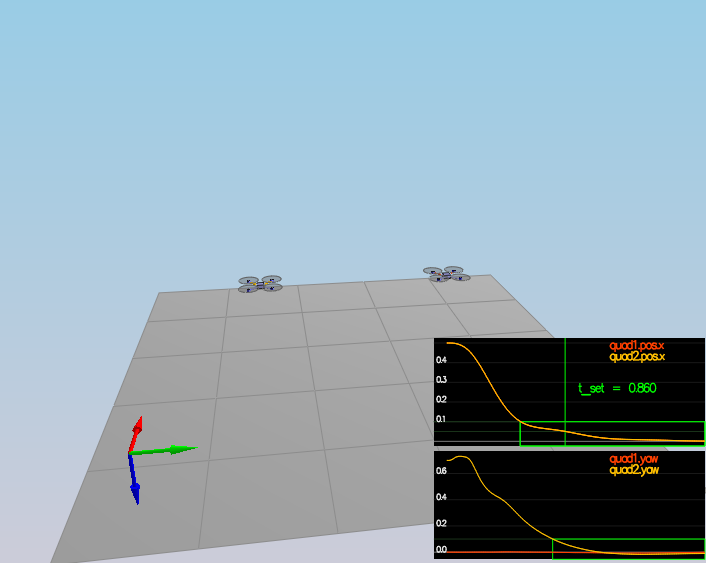
\includegraphics[width=0.5\textwidth]{./fig/scenario3.png}
\caption{\label{fig:scenario3} Scenario 3 Position/velocity and yaw angle control.}
\end{figure}

\subsection{Scenario 4: Non-idealities and robustness}

Scenario 4 simulation explores the non-ideality and robustness of controllers. Three quads are configured to move one meter forward. However, these quads have different physical characteristics:

\begin{itemize}
\item The green quad has its center of mass shifted back
\item The orange vehicle is an ideal quad
\item The red vehicle is heavier than usual
\end{itemize}

With controller gain parameters set from the previuos step, not all the quads  moving along to the target. Adding integral control in AltitudeControl() helps with the different-mass vehicle. Further tweaking the controller parameters is necessary to make all the vehicles successfully move properly  to pass the simulator test in this scenario, see Figure~\ref{fig:scenario4}.

\begin{Verbatim}[frame=single, commandchars=\\\{\}]
# Position control gains
kpPosXY = \textcolor{red}{2.5}
kpPosZ = \textcolor{red}{4}
KiPosZ = \textcolor{red}{10}

# Velocity control gains
kpVelXY = \textcolor{red}{10}
kpVelZ = \textcolor{red}{16}

# Angle control gains
kpBank = \textcolor{red}{10}
kpYaw = \textcolor{red}{2}

# Angle rate gains
kpPQR = \textcolor{red}{60}, \textcolor{red}{60}, 5
\end{Verbatim}

\begin{Verbatim}[frame=lines, label=Simulator Test Result Output, commandchars=\\\{\}]
Simulation #1278 (../config/4_Nonidealities.txt)
\textcolor{green}{PASS}: ABS(Quad1.PosFollowErr) was less than 0.100000 for at least 1.500000 seconds
\textcolor{green}{PASS}: ABS(Quad2.PosFollowErr) was less than 0.100000 for at least 1.500000 seconds
\textcolor{green}{PASS}: ABS(Quad3.PosFollowErr) was less than 0.100000 for at least 1.500000 seconds
\end{Verbatim}

\begin{figure}[ht]
\centering
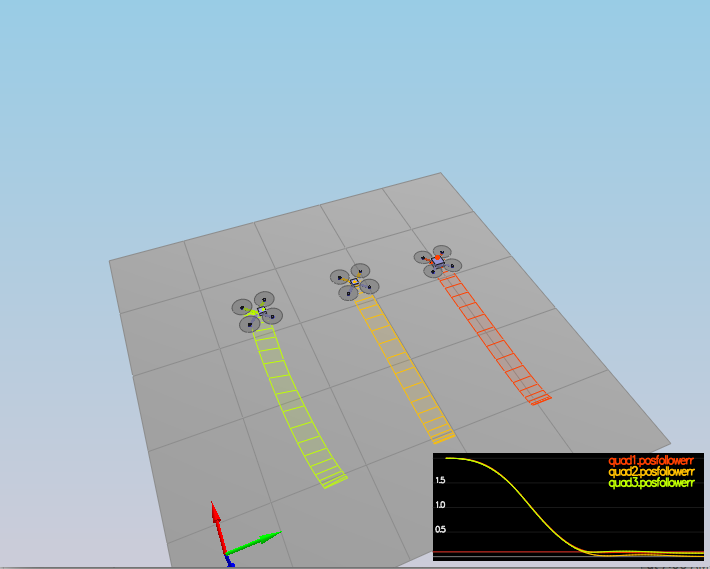
\includegraphics[width=0.5\textwidth]{./fig/scenario4.png}
\caption{\label{fig:scenario4} Scenario 4 Non-idealities and robustness.}
\end{figure}

\subsection{Scenario 5: Tracking trajectories}

Scenario 5 put all working parts of a controller together and test its performance on a yet another complex trajectory. This scenario has two quadcopters: each one follows a Figure-8 trajectory. Without any further gain tuning from previous scenario, both of the drone are able to hold to the path fairly well, shown in Figure~\ref{fig:scenario5}.

\begin{Verbatim}[frame=lines, label=Simulator Test Result Output, commandchars=\\\{\}]

Simulation #1285 (../config/5_TrajectoryFollow.txt)
\textcolor{green}{PASS}: ABS(Quad2.PosFollowErr) was less than 0.250000 for at least 3.000000 seconds
\end{Verbatim}

\begin{figure}[ht]
\centering
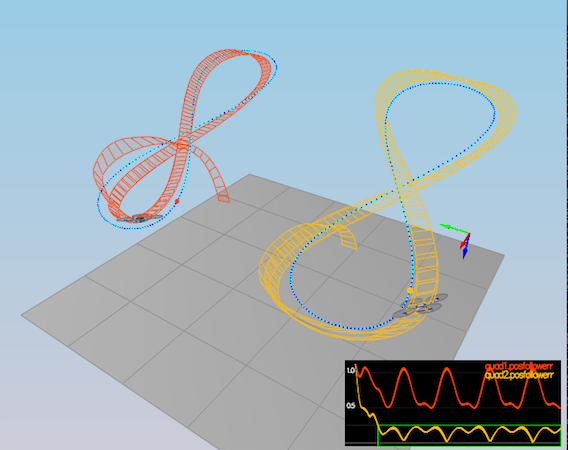
\includegraphics[width=0.5\textwidth]{./fig/scenario5.png}
\caption{\label{fig:scenario5} Scenario 5 Tracking trajectories.}
\end{figure}

\subsection{Bonus Scenario: Test many quards}

Now the C++ controller is able to fly the all provided test trajectories and passes inspection of all 5 test scenarios. Let's put it into an extra bonus test trajectory with many many quads all together (Figure~\ref{fig:scenario_test1}). It's so cool! 

\begin{figure}[ht]
\centering
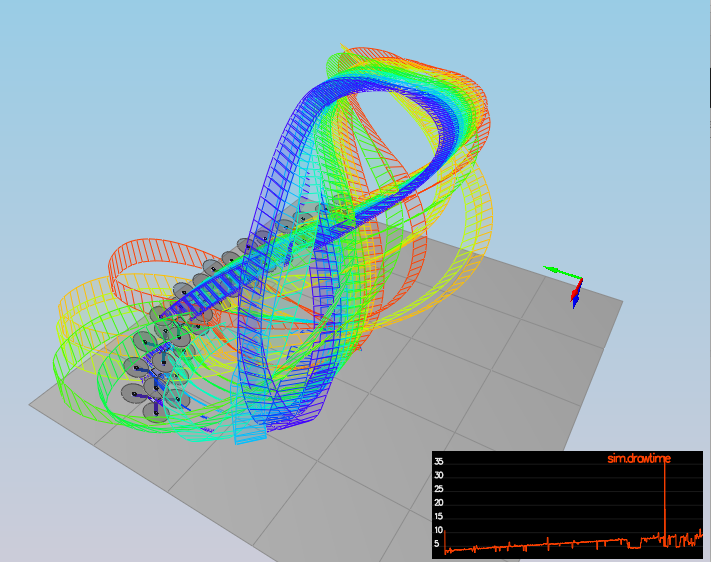
\includegraphics[width=0.5\textwidth]{./fig/scenario_test1.png}
\caption{\label{fig:scenario_test1} Bonus Scenario: Test many quards.}
\end{figure}

\end{document}